%----------------------------------------------------------------------------
\chapter{Bevezetés}

\textbf{Kontextus.} Biometrikus felhasználó azonosítás során a felhasználót saját biológiai jellemzői alapján azonosítjuk. A biometrikus azonosító rendszer a felhasználók biometrikus adatait tárolja és ezek segítségével azonosítja őket. Ezen módszer széleskörű megjelenése a mobiltelefonok fejlődésének köszönhető. Az újabb okostelefonok már képesek ujjlenyomat, arc és hang alapú azonosításra is.
\newline
\newline
A biometrikus azonosításnak számos előnye van a mai hagyományos jelszó alapú bejelentkezéssel szemben. Jelszavakat elveszíthetünk, eltulajdoníthatják tőlünk, illetve ha valaki hozzáfér az email fiókunkhoz már a kétfaktoros jelszavas autentikáció sem biztosít elegendő védelmet. A biometrikus jellemzők egyedik és fizikailag a felhasználóhoz tartoznak ezért nehéz megszemélyesíteni őket és jóval nagyobb védelmet biztosítanak a jelszavaknál. A nagyobb védelmen kívül gyorsabb és kényelmesebb használni őket, a jelszavakkal ellentétben nem kell emlékezzünk rájuk.
\newline
\newline
\textbf{Probléma.} A jelenleg elterjedt biometrikus azonosítási módszerek körében a biometrikus jel rögzítéséhez bonyolult és drága eszközökre van szükség (retinaszkenner, ujjlenyomat olvasó, digitális tábla aláíráshoz stb.).
\newline
\newline
A biometrikus azonosítási módszerek közül kevésbé elterjedt és jelenleg nagyon kutatott téma a hangalapú felhasználó azonosítás. Ennek előnye, hogy a hang rögzítéséhez nincs szükség drága vagy csak az újabb okostelefonokban található rendszerekre (retinaszkenner, ujjlenyomatolvasó), csupán egy mikrofonra és felhasználói szempontból is kényelmes.
\newline
\newline
Napról napra újabb módszerek, modellek jelennek meg, amelyek nincsenek egységesen rendszerezve, összehasonlítva. Továbbá nem létezik olyan szabad szoftver amellyel tetszőleges modellt használva szimulálhatunk egy beszélőfelismerő rendszert.
\newline
\newline
\textbf{Megvalósítás.} Dolgozatomban bemutatom a beszélőfelismerés fejlődését, megvizsgálom a mai modern neurális hálózat alapú beszélőfelismerő rendszereket, a rendelkezésre álló beszédadatbázisokat. Bemutatok részletesen két beszélőfelismerő modellt, majd meta tanítás alapú optimizációs technikákat. Végül ismertetem az általam implementált android prototípus alkalmazást hangalapú biometrikus azonosításhoz.
\newline
\newline
\textbf{Cél.} A hosszú távú cél egy olyan beszélőfelismerő rendszer létrehozása, amely segítségével összehasonlíthatjuk a különböző modellek teljesítményét, illetve egy beszélőfelismerő android kliens oldali alkalmazás létrehozása hangalapú autentikációhoz.
\newline
\newline
\textbf{Kontribúciók.} A dolgozatom a következő kontribúciókat tartalmazza:
\begin{itemize}
	\item Módosított Wavenet architektúra teljesítményének mérése beszélőfelismerésre.
	\item Mérések a voicemap modellen: VoxCeleb adatbázis, triplet loss.
	\item Android prototípus alkalmazás beszélőfelismerésre.
\end{itemize} 


\section{Biometrikus azonosítás}

A biometria az emberek fizikai jellemzőinek mérésével és elemzésével foglalkozik. Alkalmazását tekintve három területet különböztetünk meg:

\begin{itemize}
	\item Felhasználó ellenőrzés: Az azonosító rendszer a biometrikus adatot egy, korábban vetthez hasonlítja. Ez alapján dönt, hogy a felhasználó hozzáférhet-e a kívánt erőforráshoz. Ilyen egy ujjlenyomat-olvasóval ellátott mobiltelefonon a képernyőzár feloldása. A felhasználó ellenőrzés arra ad választ, hogy az illető az-e akinek mondja magát.
	\item Felhasználó azonosítás: Az azonosító rendszer a biometrikus adatot több korábban vett mintához hasonlítja és arra ad választ, hogy ki a felhasználó; azaz beletartozik-e a korábban eltárolt biometrikus adatokból álló csoportba vagy nem. Ilyen lehet például egy ujjlenyomat-leolvasóval ellátott beléptetőrendszer cégek esetében.
	\item Duplikátum detektálás: Annak ellenőrzése, hogy egy felhasználó egynél többször szerepel-e egy adatbázisban. Csalások, például szociális támogatást többször igénylők kiszűrésére használják.
\end{itemize}

Az első biometrikus azonosítási eljárás az ujjlenyomatvételen alapuló személyiségazonosítás volt, amely a modern kriminalisztika világában terjedt el, de manapság már megtalálható okostelefonokban, biometrikus beléptetőrendszerekben is.

A biometrikus azonosítást az ún. biometrikus azonosító rendszer végzi el. A folyamat során a biometrikus azonosító rendszer mintát vesz az azonosítandó egyén egy vagy több előre meghatározott fizikai jellemzőjéről, és ezekről digitális lenyomatokat képez. Az első, regisztrációs fázisban a biometrikus minta lenyomatát a rendszer egy adatbázisban eltárolja, majd később az azonosítás során az aktuális mintát összeveti a korábban rögzítettel és dönt az egyezésről. Ahhoz, hogy az ember egy fizikai jellemzőjét biometrikus adatként használhassuk, a következő elvárásokat támasztjuk vele szemben:

\begin{itemize}
	\item Általánosság: A biometrikus adattal minden egyénnek rendelkeznie kell.
	\item Egyediség: A biometrikus adatnak egyedinek kell lennie a releváns populáción belül.
	\item Állandóság: A biometrikus adat nem, vagy csak keveset változzon az idő eltetével.
	\item Mérhetőség: Az biometrikus adat az egyén részéről legyen könnyen mérhető testi adottság.
	\item Teljesítmény: A biometrikus azonosító rendszerek teljesítménye: gyorsaság, pontosság, technológia.
	\item Elfogadottság: A releváns populáción belül a mérési eljárás mennyire elfogadott (emberi méltóság megőrzése).
	\item Biztonság: Mennyire nehéz utánozni, hamisítani a biometrikus adatot?
\end{itemize}

A biometrikus adat lehet fiziológiai (DNS, arc, ujjlenyomat, írisz) vagy viselkedési (hang, írás, gesztusok). Mivel ezek az adatok statisztikai jellegűek, megbízhatóságuk változó. Minél több adat van egy mintában, annál egyedibb, és minél nagyobb a releváns populáció (eltárolt minták összessége), annál valószínűbb, hogy találunk két hasonló mintát. Ennek elkerülésére manapság terjednek a multimódusú biometrikus azonosító rendszerek, amelyek több biometrikus adatot felhasználva végzik ez az ellenőrzés, azonosítás és duplikátum detektálás feladatát. 

\section{Equal Error Rate}

Az \emph{Equal Error Rate (EER)} vagy \emph{Crossover Rate (CER)} a biometrikus rendszerek teljesítményének mérésére használatos mérőszám. Az \emph{EER} segítségével tudjuk eldönteni ellenőrzés vagy azonosítás esetén a döntési küszöbérték szintjét, amely mellett a rendszer legjobban teljesít, azaz így optimizáljuk azt. Például beszélőfelismerés esetén két hang különbségét valamekkora távolsággal jellemezzük. Ebben az esetben a küszöbérték alatt azt a távolságot értjük amely szintje alatt a két beszélőt azonosnak, fölötte különbözőnek tekintjük.
\newline
\newline
A biometrikus rendszereket három fontos mérőszámmal jellemezzük. Az FAR, az FRR és az előző kettőn alapuló EER. Az első kettőre általában angolul, a következőképpen hivatkozunk:
\begin{itemize}
	\item False Acceptance Rate (FAR): A tévesen elfogadás esetén a biometrikus rendszer beenged egy illetéktelen felhasználót, azaz hiba miatt mással azonosítja őt. A téves elfogadási ráta ennek a mértéke, a téves elfogadások számának aránya az összes elfogadáshoz képest.
	$$FAR = \frac{FA}{AA},$$
	ahol \emph{FA} a téves elfogadások száma, \emph{AA} pedig az összes elfogadás száma.
	\item False Rejection Rate (FRR): A téves visszautasítás azt jelenti, hogy az illetékes felhasználót a rendszer hiba miatt nem tudja azonosítani. A téves visszautasítási ráta a téves visszautasítások számának aránya az összes visszautasításhoz képest.
	$$FRR = \frac{FA}{AA},$$
	ahol \emph{FR} a téves visszautasítások száma, \emph{AR} pedig az összes visszautasítás száma.
\end{itemize}
Az EER az a pont, ahol az FAR értéke megegyezik az FRR-el.
\newline
\newline
A biometrikus rendszerek karakterisztikáját a \ref{fig:eer} ábra szemlélteti. Vegyük a beszélőazonosító rendszer példáját. Látható, hogy a döntési küszöb növelése (mekkora távolság esetén tekintjük azonosnak a két beszélőt) esetén az \emph{FAR} nő és az \emph{FRR} csökken. Ez normális, mert ilyenkor megengedőbbek vagyunk, nagyobb távolság esetén is azonosnak tekintjük a két beszélőt, így több olyan eset lesz amikor két beszélő különbözik, a rendszer mégis azonosnak tekinti őket és kevesebb olyan amikor két beszélő azonos és a rendszer mégis visszautasít. 
\newline
\newline
Ha a küszöböt csökkentjük szigorúbb lesz a rendszer, sokkal kevesebb téves elfogadás lesz, de a szigorúság miatt megnő a téves viszautasítások száma.
\newline
\newline
Az EER a két grafikon metszéspontjában található, ahol FAR és FRR értéke minimális és optimális (az optimizálás alatt érthetjük a kettő szorzatát). Az EER a vízszintes tengelyen megadja az optimális küszöbértéket, a függőlegesen pedig egy hiba rátát. Ez az FRR és FAR hiba rátája, mivel a kettő ebben a pontban megegyezik.

\begin{figure}[!ht]
	\centering
	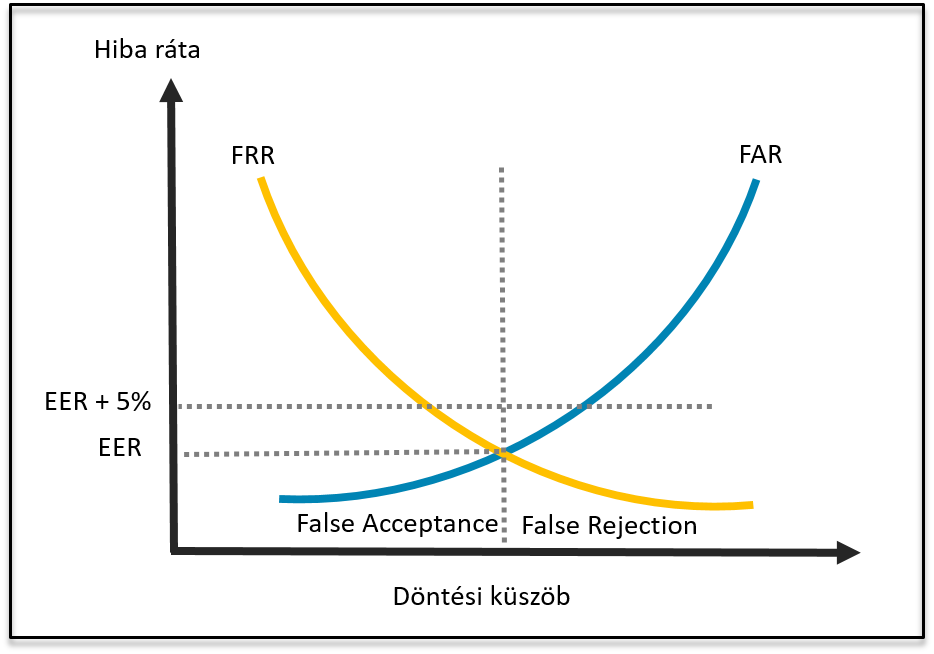
\includegraphics[width=150mm, keepaspectratio]{figures/eer.png}
	\caption{Biometrikus rendszerek karakterisztikája.}
	\label{fig:eer}
\end{figure}



\section{Beszélőfelismerés}

Az emberi kommunikáció során fontos feladat a beszélő partner felismerése. A telekommunikációs technológia fejlődése miatt elterjedt a telefonon vagy interneten történő hangalapú kommunikáció; a telefonos felhasználófelismerés mint biometrikus azonosítási módszer megjelent már banki alkalmazásokban, call centerekben és az elektronikus kereskedelemben is (mobiltelefonos vásárlás). Az elektronikus kommunikáció során sokszor csak a beszélő hangjára hagyatkozhatunk, az alapján ismerhetjük fel az illetőt. A beszélőfelismerést háromféle módon végezhetjük:

\begin{itemize}
	\item Naiv beszélőfelismerés: Az emberi, naiv beszélőfelismerés során az ismerős hangokat meglepően nagy pontossággal ismerjük fel.
	\item Törvényszéki beszélőfelismerés: A törvényszéki szakértői vizsgálat eredménye.
	\item Automatikus beszélőfelismerés: A beszélőfelismerést számítógépes rendszer végzi.
\end{itemize}

A beszélőfelismerés alatt három szűkebb fogalmat értünk. Ha a folyamat során az ismeretlen beszélőről azt ellenőrizzük, hogy az-e akinek állítja magát beszélő ellenőrzésről van szó. Beszélő szegmentáláskor a hangmintát homogén csoportokra bontjuk a beszélő személye alapján. Végül beszélő azonosításról beszélünk, ha az illető hangját rögzített hangok egy csoportjával vetjük össze és azt szeretnénk eldönteni, hogy melyikhez hasonlít a legjobban. Utóbbi felveti a kérdést, hogy mi történik ha a beszélő nem tagja a csoportnak. 

Emiatt megkülönböztetjük a nyitott és zárt halmazú beszélőazonosítást. Utóbbi esetén csak olyan beszélőket ismerünk fel, akikről van hangminta az adatbázisban, míg az előbbinél ismeretlen beszélők is megjelenhetnek, így ezt is kezelni kell.

A beszélőfelismerés továbbá lehet szöveg-függő és szöveg-független attól függően, hogy a felismerő rendszer egy előre meghatározott mondatot vár, vagy bármilyen hangminta alapján működik.

\section{Az automatikus beszélőfelismerés története}

Az automatikus beszélőfelismerést egy számítógépes program végzi emberi beavatkozás nélkül. Az első automatikus beszédfelismerő rendszert a Texas Instruments fejlesztetése volt és 1977-ben publikálták. A rendszer szövegfüggő beszélőellenőrzésre volt képes és az évek során a téves elutasítási és elfogadási rátája 1$\%$ alatt maradt. A hetvenes évek óta a a beszélőazonosító és ellenőrző rendszerek rengeteget fejlődtek kezdve a vektor kvantálástól kezdve a GMM modelleken át a mély neurális hálókig. 

\begin{figure}[!ht]
	\centering
	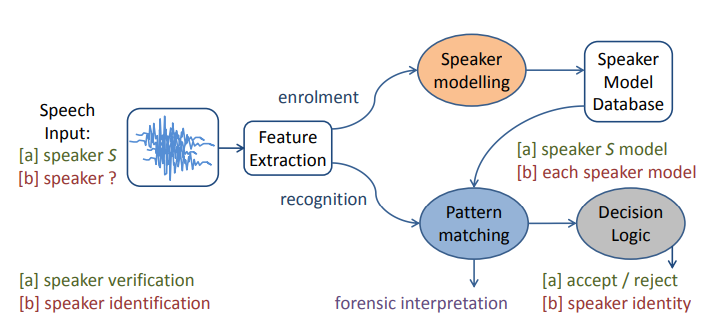
\includegraphics[width=150mm, keepaspectratio]{figures/automatic_speaker_recognition.png}
	\caption{Automatikus beszélőfelismerő rendszer architektúrája.}
	\label{fig:automatic_speaker_recognition}
\end{figure}

Az automatikus beszélőfelismerő általános működését az alábbi (!) ábra szemlélteti. A beszélő-ellenőrzés és beszélőazonosítás során is az első lépés rögzített \emph{jellemzők kinyerése}. Ezután az első, \emph{tanító fázisban} referencia modelleket készítünk az egyes beszélőkhöz a jellemzők alapján, amelyeket eltároljuk a beszélő adatbázisban. Beszélő-ellenőrzés esetén ebben a fázisban egy küszöbérték is meghatározásra kerül. \emph{Teszt fázisban} a rendszer kinyeri ugyanazokat a jellemzőket az aktuális hangmintából, majd \emph{jellemző összehasonlítás} történik.

\begin{enumerate}
	\item beszélő-ellenőrzés esetén megkeresi az ellenőrizendő személyhez tartozó modellt az adatbázisban és összehasonlítja az aktuális jellemzőkkel. Ha az eredmény a küszöbszint felett van, a rendszer egyezést mutat.
	\item beszélőazonosítás esetén az aktuális jellemzőket az összes modellel összehasonlítja, majd a legjobb egyezés mellett dönt. 
\end{enumerate}

\subsection{Jellemző kinyerés}
A jellemző kinyerés célja a dimenzió csökkentése és a beszélőspecifikus információk kinyerése. Mivel a beszéd komplex jel, a beszélő azonosítása szempontjából felesleges információkat is hordoz. Ilyen például a környezet és a csatorna zaja. A kinyert jellemzőket a hangminta terjedelme alapján osztályozzuk. \emph{Rövidtávú jellemzők} a 20-30 ms-os keretekből kinyert mel-frekvenciás és lineáris prediktív kepsztrális együtthatók (MFCC és LPCC). A \emph{prozódikus jellemzők} kinyerése 100 ms-os terjedelemben történik és a beszéd ritmusát, a hangmagasságot és a sebességet jellemzik. A hosszútávú jellemzőket a jel akár perc hosszú kereteiből nyerjük ki. Ezek képesek reprezentálni a beszélő akcentusát illetve a szavak szemantikáját és az idiolektust.

A beszélőfelismerő rendszerek teljesítményét javította, ha a jellemzőket csak
a hangminta azon részeiből nyerték ki, amikben beszéd is volt. Erre alkalmazott technika a \emph{Voice Activation Detection} (\emph{VAD}).

\subsection{Jellemző normalizálás}

Jellemzőkinyerés során próbáljuk kiszűrni a beszélő szempontjából értékes részéket, ugyanakkor nincs tökéletes jellemző, amely ne változna a környezet hatására. Ezt a változást segítik minimalizálni a normalizálási módszerek.

\subsection{A beszélőfelismerő modellek története}

Kezdetben a vektor kvantálás volt az elterjed modellezési módszer, amit később a \emph{Gaussian Mixture Model} (\emph{GMM}) váltott fel. A GMM egy adathalmazt több normális eloszlás keverékeként ír le és képes nem felügyelt módon klaszterezni az adatokat. Egy beszélőhöz egy valószínűségi sűrűségfüggvényt rendel, amely különböző pontokban kiértékelve (például teszt fázisban a beszélőtől kinyert jellemzők) egy valószínűséget ad a két beszélő hasonlóságára.

A GMM megközelítés főleg beszélőazonosításra alkalmas. Beszélő-ellenőrzéshez szükség volt egy másik modellre is, ami képes leírni minden más beszélőt az ellenőrizendőn kívül. Erre adott megoldást az \emph{Universal Background Model} (\emph{UBM}). Később jobb teljesítményt értek el, ha a teszt fázisban a beszélőkkel először UBM modelleket tanítottak és ezekből származtattak GMM-eket. Ezt nevezik GMM-UBM módszernek.

Mivel a tanító és teszt hangminták eltérő hosszúságúak lehetnek, szükség volt egy fix hosszúságú reprezentációra, ezt oldották meg a GMM szupervektorok, amelyeket az akkori megközelítés szerint szupport-vektor gépekkel vagy faktoranalízissel használtak.

Az utóbbi két módszer előnyeit kombinálva megszületett az $i-vektorok$, amelyet követve eljutunk a mai state-of-the-art módszerhez, a mély neurális hálózatokhoz (DNN).

\section{Korábbi eredmények}



\begin{table}[!ht]
	\resizebox{\textwidth}{!}{%
	\begin{tabular}{*7l} \toprule
		\bfseries Szerző (év)
		& \bfseries Szervezet
		& \bfseries Adatbázis
		& \bfseries Módszer
		& \bfseries Jellemzők
		& \bfseries \begin{tabular}{@{}l@{}} Hang \\ típusa \end{tabular}
		& \bfseries Pontosság \\ \midrule
		
		\begin{tabular}{@{}l@{}} Douglas A. Reynolds  \\  (1995) \end{tabular}
		& \begin{tabular}{@{}l@{}} Lincoln  \\  Laboratory \end{tabular}
		& 49
		& MFCC 
		& \begin{tabular}{@{}l@{}} rövid \\ kifejezések \end{tabular} 
		& telefon 
		& 96.8 \% \\
		
		\begin{tabular}{@{}l@{}} Rabah W.  \\  (2004) \end{tabular}
		& \begin{tabular}{@{}l@{}} King Abdulaziz  \\  University \end{tabular}
		& 20
		& \begin{tabular}{@{}l@{}} SVD-alapú   \\  algoritmus \end{tabular}
		& LPC/Cepstral
		& iroda
		& 94 \% \\
		
		\begin{tabular}{@{}l@{}} Yang Shao  \\  (2008) \end{tabular}
		& \begin{tabular}{@{}l@{}} Ohio State  \\  University \end{tabular}
		& 34 
		& GFCCs 
		& hallási jellemzők
		& telefon
		& \~{}99.33 \% \\
		
		\begin{tabular}{@{}l@{}} P. Krishnamoorthy  \\  (2011) \end{tabular}
		& TIMIT
		& 100 
		& GMM-UBM 
		& MFCC
		& labor
		& 80 \% \\
		
		\begin{tabular}{@{}l@{}} Alfredo Maesa  \\  (2012) \end{tabular}
		& Voxforge.org
		& 250 
		& MFCC 
		& \begin{tabular}{@{}l@{}} spektrális \\ jellemzők \end{tabular} 
		& \begin{tabular}{@{}l@{}} beszéd- \\ adatbázis \end{tabular} 
		& > 96 \% \\

		\begin{tabular}{@{}l@{}} Sharada V. Chougule  \\  (2015) \end{tabular}
		& \begin{tabular}{@{}l@{}} Finolex Academy  \\  of Management \\ and Technology \end{tabular}
		& 97 
		& NDSF 
		& spektrális
		& labor
		& \~{}98-100 \% \\
		
	\bottomrule
	\end{tabular}}
	\centering
	\caption{Korábbi eredmények szövegfüggetlen beszélőazonosítás terén.}
	\label{fig:timit-dialects}
\end{table}

\newpage

\section{Modern beszélőfelismerés}

A következő fejezetben bemutatom a 2017-2019-ben publikált korszerű beszélőfelismerő rendszereket és hogy milyen eredményeket értek el. Mivel ez a kutatási terület jelenleg népszerű és folyamatosan újabb eredményeket érnek el, a bemutatott rendszereket a hivatkozások száma, a dátum és a \emph{www.paperswithcode.com} oldal rangsorolása alapján választottam ki.
\newline
\newline
Az eredmények általános összehasonlítása több ok miatt is nehéz feladat. A cikkekben a legjobb eredmények feltüntetése miatt relatív eredményeket tartalmaznak egy-egy korábban
publikált rendszerhez képest. Ezen kívül változik, hogy zárt vagy nyílt-halmazú beszélőfelismerés, beszélő-ellenőrzésről van-e szó, maga a teszthalmaz nehézsége: etnikai, nemi, foglalkozásbeli diverzitás, a hangminták hossza, a hangfelvétel minősége, van-e irreleváns zaj, stb. Továbbá
a legtöbb cikk nem biztosít letölthető modellt, konfigurációt, szkripteket az előfeldolgozáshoz, így
azonos környezethez reprodukálni kellene azokat.


\subsection{Deep Speaker: an End-to-End Neural Speaker Embedding System (2017)}

A Deep Speaker egy neurális hálózatokon alapuló embedding rendszer. Az \emph{embedding} kifejezés alatt valamilyen leképzést értünk. Például amikor hangokból hangvektorokat készítünk. A rendszer a hangmintákat egy hipergömbre vetíti, ahol azoknak a hasonlóságát koszinusz távolsággal méri.
\newline
\newline
A leképzések előnye, hogy felhasználástól függetlenek, módszertől függően használhatók beszélőazonosításra, identifikációra és diarizációra is. 
\newline
\newline
Jellemző kinyerésre ResNet és GRU (LSTM változat) architektúrákkal próbálkoztak. Tanításhoz \emph{triplet loss} veszteséget használtak, és a hangvektorok között koszinusz távolságot számoltak.
\newline
\newline
A Deep Speaker által elért eredményeket a korábbi legkorszerűbb \emph{i-vektoros} rendszerekhez mérték.
Ezeknek az általános felépítése a következőképpen néz ki:
\begin{itemize}
	\item Statisztikák gyűjtése
	\item i-vektorok leképzése (jellemző kinyerés)
	\item osztályozás (PLDA)
\end{itemize} 
Ezek a rendszerek \emph{GMM-UBM} modellt használtak a statisztikák kinyerésére, amiket jellemzőkkel (pl. MFCC) optimalizáltak. A GMM-UBM helyett később
DNN alapú megoldással is próbálkoztak. A GMM-UBM kimeneteként kapott
sokdimenziós statisztikákat ezután alacsony dimeziójú i-vektorokká alakítják, amit aztán PLDA modellel osztályoznak és verifikációra használják.
Jelenleg a mai korszerű rendszerek az első két lépést összevonják és CNN-eket használnak alacsony dimenziós jellemzőkinyerésre.
\begin{table}[!ht]
	\begin{tabular}{*3l} \toprule
		\bfseries Rendszer & \bfseries EER (\%) & \bfseries ACC (\%) \\ \midrule
		DNN i-vector baseline & 13,79 & 51,72 \\
		\rowcolor{gray!10}
		ResCNN, softmax & 6,13 & 81,95 \\
		ResCNN, triplet & 2,69 & 86,21 \\
		\rowcolor{gray!10}
		ResCNN, softmax (pre-train) + triplet & 2,23 & 90,53 \\
		GRU, softmax & 5,42 & 83,05 \\
		GRU, triplet & 3,23 & 84,19 \\
		\rowcolor{gray!10}
		GRU, softmax (pre-train) + triplet & 2,77 & 89,50 \\
		\bottomrule
		\hline
	\end{tabular}
	\centering
	\caption{Mandarin nyelvű szöveg-független azonosítás eredményei tanításra és tesztelésre a Train50k és Eva200 adathalmazokat használva.}
	\label{fig:deep-speaker-independent-mandarin-results}
\end{table}

A legjobb architektúrának a \emph{ResCNN} bizonyult softmax előtanítással és triplet lossal tanítva. Ezzel a \ref{fig:deep-speaker-independent-mandarin-results} szerint Eva200 adathalmazon \emph{90,53\%}-os eredményt értek el. A Train50k, Train250k és Eva200k az UID adathalmaz részei.

\begin{table}[!ht]
	\begin{tabular}{*3l} \toprule
		\bfseries Rendszer & \bfseries EER (\%) & \bfseries ACC (\%) \\ \midrule
		ResCNN on Train50k & 2,23 & 90,53 \\
		\rowcolor{gray!10} 
		ResCNN on Train250k & 1,83 & 92,58 \\
		GRU on Train50k & 2,77 & 89,50 \\
		\rowcolor{gray!10} 
		GRU on Train250k & 2,35 & 90,77 \\
		\bottomrule
		\hline
	\end{tabular}
	\centering
	\caption{Szöveg-független azonosítás eredményei.}
	\label{fig:deep-speaker-independent}
\end{table}

A \ref{fig:deep-speaker-independent} szerint pedig nagyobb adathalmazzal való tanítás nagyobb pontosságot és alacsonyabb EER-t eredményezett. A legjobb eredményt a RestCNN-el érték el Train250k-val tanítva.
\newline
\newline
Az eredmények a korábbi i-vektoros rendszerekhez képest a Deep Speaker 50\% csökkentette az EER-t, és pontosságban 60\%-os javulást ért el.

\subsection{Speaker Recognition from Raw Waveform with SincNet (2018)}

A SincNet is a korábban használt i-vektoros rendszerek helyett mutat be egy új CNN hálózatot. A CNN-ek előnye, hogy a korábban használt kézzel fabrikált jellemzők (pl. MFCC) helyett a hálózat maga tanulja meg a hang alacsony szintű reprezentációját nyers hullámformákból. Mivel a cikk a CNN-t kiegészíti hangszűrőkkel és a jelfeldolgozásban használatos fogalmakat használ, először ismertetem ezeket:
\begin{itemize}
	\item Beszéd frekvencia: Egy periodikus hullámforma esetében a frekvencia a periódusidő reciproka, azza megmondja, hogy egységnyi idő alatt hány periódus ment végbe. Az emberi hang esetében a komplex hullámforma Fourier analízissel felbontható trigonometrikus (periodikus) függvények összegére. A Fourier transzformáció segítségével az idő-amplitúdó doménből frekvencia-amplitúdót képzünk, így a frekvencia komplex jel esetén és értelmet nyer.
	\item Sávszélesség: Hang esetében általánosan a legalacsonyabb és legmagasabb frekvencia közötti különbség.
	\item Cutoff frekvencia: A hangszűrők legfontosabb paramétere. Például aluláteresztő szűrő esetében a cutoff fölötti frekvenciákat a szűrő tompítja, nem engedi át.
	\item Band pass filter: Olyan szűrő, ami csak a cutoff frekvencia környezetében lévő frekvenciákat engedi át (egy alul -és felüláteresztő szűrő kombinációja).
\end{itemize} 
\ \\
\newline
\newline
A SincNet egy új CNN architektúra, amelyben az első réteg ún. paraméterezhető sinc függvényekkel van kiegészítve, amelyek band pass szűrőket implementálnak.
\newline
\newline
A korábban használt kézzel fabrikált jellemzők, mint az MFCC vagy FBANK esetében semmi sem garantálja, hogy optimálisak minden beszélőfelismerő feladatra. A cikk szerint lehetséges, hogy ezek a jellemzők nem veszik figyelembe a hangmagasságot és a formánsokat. A feltevésük szerint hullámforma feldolgozásánál a legfontosabb a CNN első rétege. Ezért a SincNet a hullámformákat sinc függvényekkel konvolválja, amelyek paraméterei az alacsony és magas cutoff frekvencia.

\begin{figure}[!ht]
	\centering
	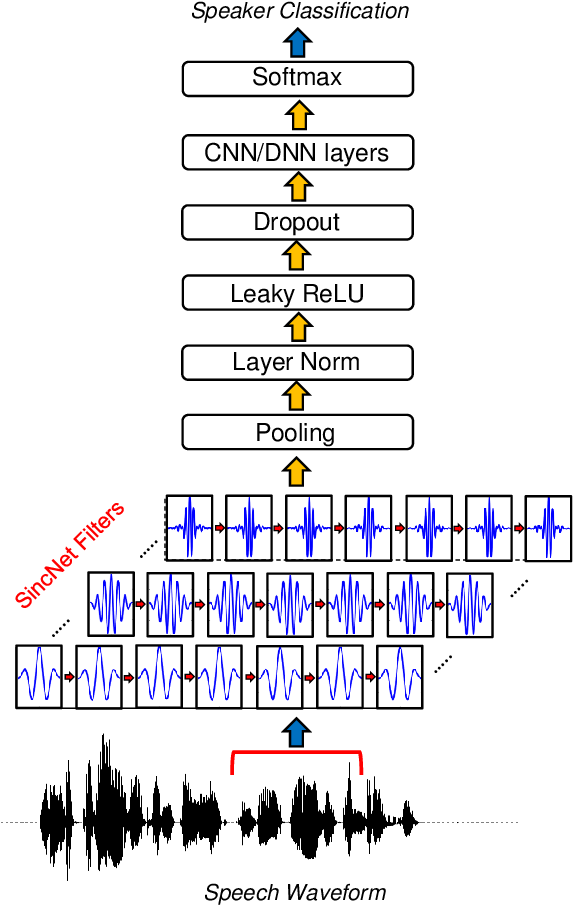
\includegraphics[width=120mm, keepaspectratio]{figures/sincnet-nn.png}
	\caption{SincNet architektúra.}
	\label{fig:sincnet-nn}
\end{figure}
\ \\
\newline
\newline
A SincNetet a TIMIT (462 beszélő) és Librispeech (2484 beszélő) adatbázisokkal tanították.
A beszédminták elejéről a szüneteket eltávolították, és LibriSpeech esetén azokat a mintákat, amelyek tartalmaztak legalább 125 ms hosszú szünetet, annak mentén feldarabolták. A TIMIT adatbázisnál egy beszélőtől 5 mintával tanítottak és 3 mintával teszteltek, míg LibriSpeechnél véletlenszerűen választottak 12-16 másodperces mintákkal tanítottak és 2-6 másodpercesekkel teszteltek.
\newline
\begin{table}[!ht]
	\begin{tabular}{*3l} \toprule
		\bfseries Rendszer & \bfseries TIMIT & \bfseries LibriSpeech \\ \midrule
		DNN-MFCC & 0,99 & 2,02 \\
		\rowcolor{gray!10} 
		CNN-FBANK & 0,86 & 1,55 \\
		CNN-Raw  & 1,65 & 1,00 \\
		\rowcolor{gray!10} 
		SINCNET & 0,85 & 0,96 \\
		\bottomrule
		\hline
	\end{tabular}
	\centering
	\caption{Szöveg-független azonosítás eredményei adatbázisok szerint.}
	\label{fig:sincnet-identification}
\end{table}
\ \\
A \ref{fig:sincnet-identification}-es táblázat a CER (Classification Error Rate [\%]) hiba rátát mutatja. E szerint a SincNet jobban teljesít az MFCC, FBANK és nyers hullámformákkal tanított CNN-eknél mindkét adatbázis esetében, bár látható, hogy a sima CNN és a SincNet között minimális a különbség.
\newline
\begin{table}[!ht]
	\begin{tabular}{*3l} \toprule
		\bfseries Rendszer & \bfseries d-vector & \bfseries DNN-class \\ \midrule
		DNN-MFCC & 0,88 & 0,72 \\
		\rowcolor{gray!10} 
		CNN-FBANK & 0,60 & 0,37 \\
		CNN-Raw  & 0,58 & 0,36 \\
		\rowcolor{gray!10} 
		SINCNET & 0,51 & 0,32 \\
		\bottomrule
		\hline
	\end{tabular}
	\centering
	\caption{Szöveg-független ellenőrzés (verifikáció) eredményei.}
	\label{fig:sincnet-verification}
\end{table}
\ \\
\newline
A SincNettel nem jellemző vektorokat képeztek és a köztük lévő távolságot használták a hasonlóság mérésére, hanem osztályozással használják. Ebben az esetben zárt-halmazú beszélőazonosításról beszélünk. Ez sokkal kevésbé flexibilis, mert új beszélő esetén mindig újra kell tanítani a hálózatot, de cserébe jobb teljesítményre képes. A \ref{fig:sincent-verification} ábrán egy d-vector nevű hangvektorokat képző neurális hálózatot hasonlítottak össze a SincNettel. Beszélőellenőrzés esetén a SincNet sokkal jobb EER-t ért el.
\newpage
\subsection{VoxCeleb2: Deep Speaker Recognition (2018)}

A VoxCeleb1 és VoxCeleb2 nagy méretű, beszélőfelismerés céljából készült adatbázisok. Az előbbi több mint 1000, utóbbi pedig több mint 6000 hangmintát tartalmaz hírességektől. Az adatbázisok felépítésének részleteit a \ref{voxceleb1} és \ref{voxceleb2} fejezetek ismertetik. Mindkét adatbázissal végeztek méréseket különböző neurális hálózatokkal, de a legjobb eredményeket illetve nyílt-halmazú beszélőfelismerést a VoxCeleb2-vel érték el.
\newline
\newline
Bemutatják a VGGVox nevű CNN alapú neurális hálózatot, amelyet spektrogramokkal tanítottak és hangvektorokat hoz létre. Előnye ennek a megoldásnak, hogy nyílt-halmazú beszélőfelismerésre használható, új beszélő esetén nem szükséges újra tanítani a hálózatot. 
\newline
\newline
Módosított VGG-M és ResNet architektúrákkal kísérleteztek. A modelleket contrastive loss veszteségfüggvénnyel tanították és előtanításra egy softmax réteget használtak keresztentrópiával, ami javította a modell teljesítményét. Tanító adathalmaznak a VoxCeleb2 adatbázist használták és a tesztelést a VoxCeleb1-el végezték. A méréseket EER és a \ref{eq:cdet} detektálási költség függvény szerint értékelték ki,

\begin{equation} \label{eq:cdet}
C_{det} = C_{miss} \cdot P_{miss} \cdot P_{target} + C_{fa} \cdot P_{fa} \cdot (1 - P_{target})
\end{equation}

ahol \emph{C\_miss} és \emph{C\_fa} alkalmazás specifikus paraméterek a hamis negatív és hamis pozitív hibák költsége, \emph{P\_miss} és \emph{P\_fa} pedig a hibák előfordulásának valószínűségét jelzik. \emph{P\_target} annak a valószínűsége, hogy a rendszer két olyan mintát hasonlít össze, amely egy embertől származik.
\newline
\begin{table}[!ht]
	\begin{tabular}{*4l} \toprule
		\bfseries Rendszer & \bfseries Tanítóhalmaz & \bfseries $C_{min}^{det}$ & \bfseries EER \\ \midrule
		I-vectors + PLDA & VoxCeleb1 & 0,73 & 8,8 \\
		VGG-M (Softmax) & VoxCeleb1 & 0,75 & 10,2 \\
		VGG-M & VoxCeleb1 & 0,71 & 7,8 \\
		VGG-M  & VoxCeleb2 & 0,609 & 5,94 \\
		ResNet-34 & VoxCeleb2 & 0,549 & 4,83 \\
		ResNet-50 & VoxCeleb2 & 0,429 & 3,95 \\
		\bottomrule
		\hline
	\end{tabular}
	\centering
	\caption{Beszélő ellenőrzés (verifikáció) eredményei.}
	\label{fig:sincnet-verification}
\end{table}

\newpage

\subsection{Utterance-level Aggregation for Speaker Recognition in the Wild (2019)}

A cikk két fő témája egy olyan neurális hálózat létrehozása, amely képes különböző hosszúságú hangmintákból jellemző vektorokat képezni és olyan hangminták vizsgálata amelyek irreleváns zajokat is tartalmaznak.

\begin{figure}[!ht]
	\centering
	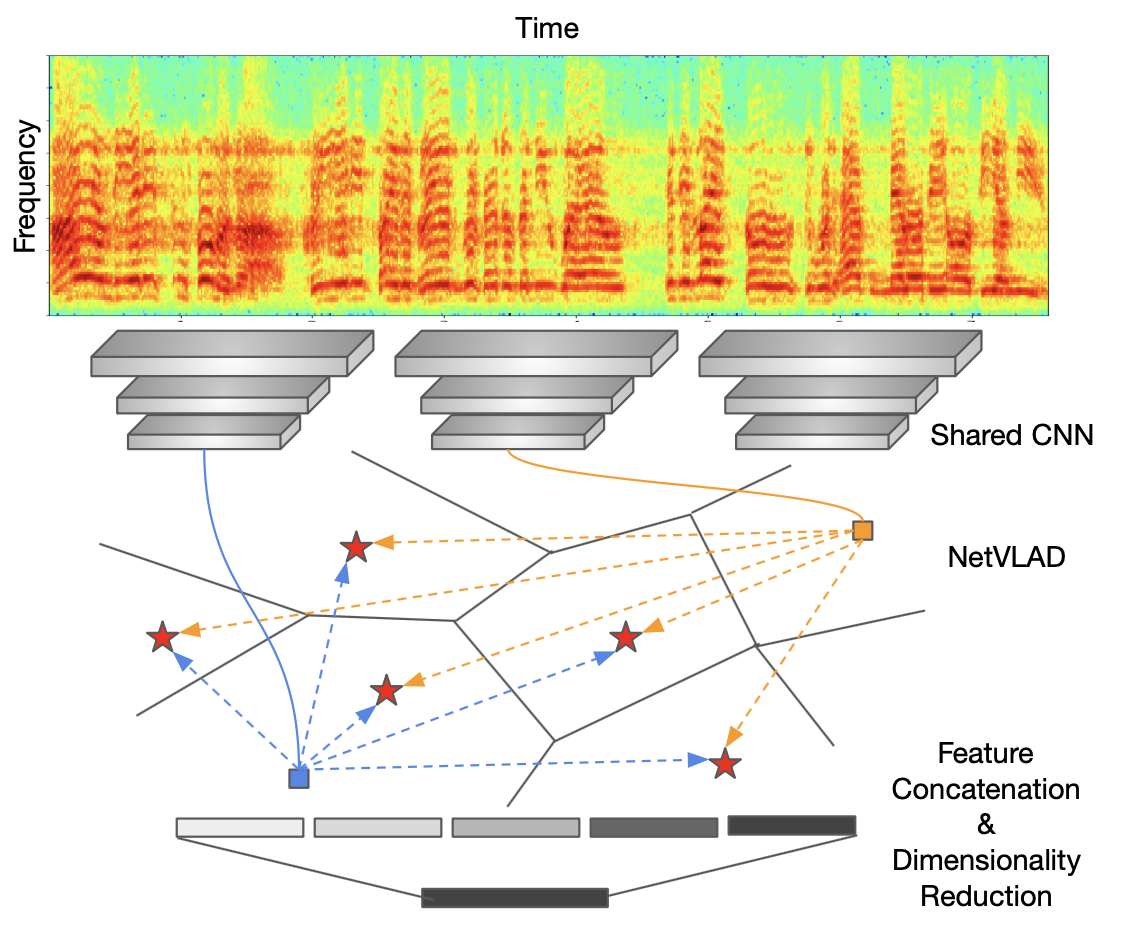
\includegraphics[width=150mm, keepaspectratio]{figures/frame-cnn.png}
	\caption{Neurális hálózat architektúra.}
	\label{fig:frame-cnn}
\end{figure}
\ \\
\newline
\newline
A hálózat három részből áll. Először egy módosított ResNet architektúrát használnak a keretszintű vektorok előállítására spektrogramokból. Az ábrán látható megosztott CNN-t hívjuk trönk hálózatnak. A keretszintű vektorok aggregálását a NetVLAD illetve GhostVLAD (Vector of Locally Aggregated Descriptors módszeren alapuló) hálózatokkal végzik. Legvégül egy FC (Fully Connected) réteget használnak a dimenzió 512-re csökkentésére.
\newline
\newline
A teljes modell end-to-end tanítására a VoxCeleb2 adatbázist használták és tesztelésként beszélőellenőrzést (verifikációt) mértek a VoxCeleb1-en.
\begin{figure}[!ht]
	\centering
	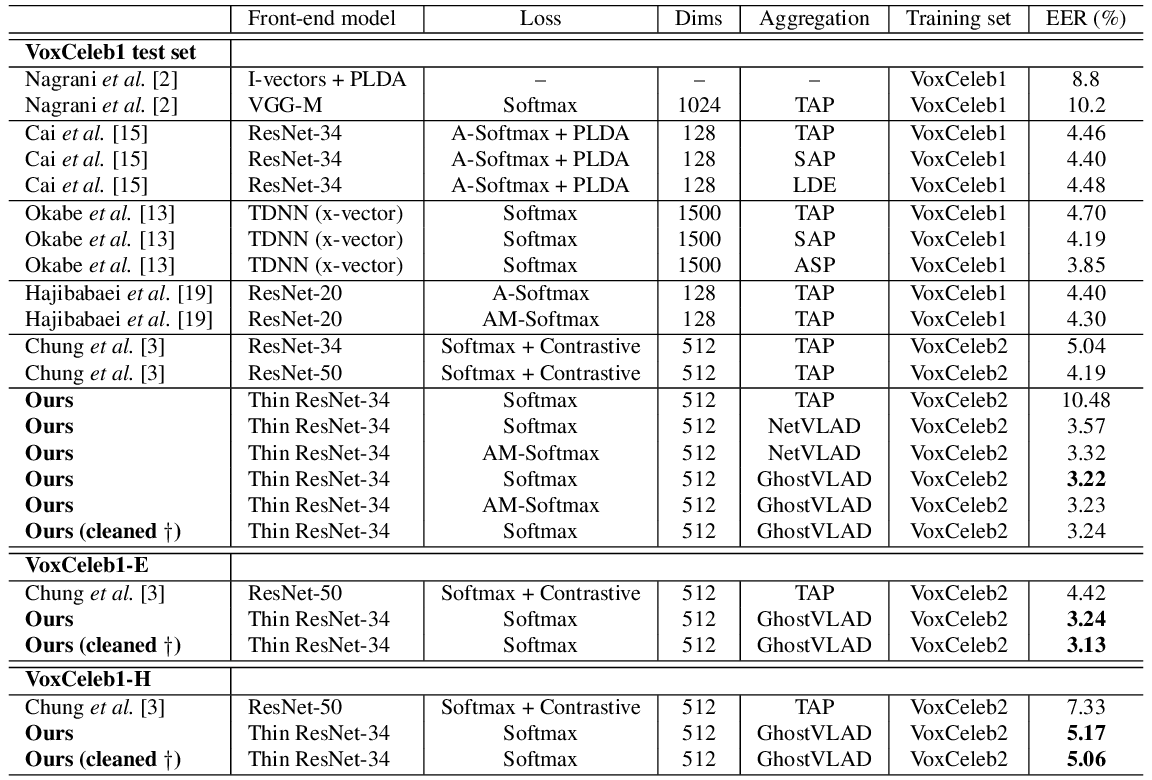
\includegraphics[width=150mm, keepaspectratio]{figures/frame-cnn-results.png}
	\caption{Neurális hálózat architektúra.}
	\label{fig:frame-cnn-results}
\end{figure}
\ \\
A \ref{fig:frame-cnn-results} táblázat mutatja a verifikációval mért EER-eket az akkori legkorszerűbb rendszerekkel szemben. Az addigiaknál lényegesen jobb EER-t értek el ezzel a módszerrel.


